\documentclass[a4paper,10pt,fleqn]{article}

\usepackage{src/common/layout}
\usepackage{float}
\usepackage{longtable}			% Tabellen 
\usepackage{booktabs}			% Tabellen
% Spezialpakete
\usepackage{fp}
\usepackage{tikz}
\usepackage{xcolor}
% TikZ-Bibliotheken
\usetikzlibrary{arrows}
\usetikzlibrary{shapes}
\usetikzlibrary{decorations.pathmorphing}
\usetikzlibrary{decorations.pathreplacing}
\usetikzlibrary{decorations.shapes}
\usetikzlibrary{decorations.text}
\newboolean{STANDALONE}
\setboolean{STANDALONE}{false}

\newboolean{EMBED}
\setboolean{EMBED}{false}


\setboolean{STANDALONE}{true}

\newcommand{\EtPath}{src/Stepper}
\newcommand{\BIBLIOGRAPHY}{src/common/ET-Gruppe_Source}
\newcommand{\DasAndereTeam}{T27}
\newcommand{\BLDCTeams}{T27 und T32}
\newcommand{\BLDCcollab}{Dieses Kapitel ist eine Zusammenarbeit der Gruppen \BLDCTeams. }

\begin{document}
	\begin{titlepage}

\begin{center}

% Oberer Teil der Titelseite:
%\includegraphics[width=0.15\textwidth]{./logo}\\[1cm]    
\textsc{\LARGE Produktentwicklung 1}\\[1.5cm]

\textsc{\Large Hochschule Luzern\\
    ~\\
    Technik \& Architektur}\\[0.5cm]

\vfill{}

% Title
\newcommand{\HRule}{\rule{\linewidth}{0.5mm}}
\HRule \\[0.4cm]
{   \Huge \bfseries Stepper Treiber\\
        ~\\
        \large Konzeptbeschreibung}\\[0.4cm]

\HRule \\[1.5cm]

% Author and supervisor
\begin{minipage}{0.4\textwidth}
    \begin{flushleft} \large
        \emph{Autorin:}\\
        Bettina \textsc{Wyss}\\
    \end{flushleft}
\end{minipage}
\hfill
\begin{minipage}{0.4\textwidth}
    \begin{flushright} \large
        \emph{Projektgruppe:} \\
        PREN-ET
    \end{flushright}
\end{minipage}

\vfill{}
\vfill{}
\vfill{}

% Unterer Teil der Seite
{\large Horw\\ \today}

\end{center}

\end{titlepage}

	\tableofcontents
	\newpage
	\ifSTANDALONE
\section{Hardware}
\fi
\ifEMBED
\subsection{Hardware}
\fi
Die Elektrotechnik-Studierenden aus mehreren Gruppen haben sich
zusammengeschlossen um gemeinsame Probleme anzugehen. Dabei handelt es sich
um die benötigte Hard- und Software, um Motoren anzusteuern
und gegebenenfalls zu regeln. In diesem Zusammenschluss wurden drei Gruppen
gebildet, um Lösungen für DC-, Stepper- und Brushless-Motoren auszuarbeiten.
Die Idee besteht darin, dass nicht jede Gruppe für dasselbe Problem wo
möglich denselben Lösungsansatz verfolgt, sondern die Ressourcen kombiniert,
Synergien nutzt um eine bessere Lösung zu erarbeiten. Auf diese Weise kann
das Team übergreifende Arbeiten im Rahmen der PREN erlernt und
geübt werden. Somit wird Idee der Interdisziplinarität im erweiterten Sinn
Rechnung getragen. Die Gruppen und deren Mitglieder sind in der Tabelle 
\ref{tab:pren-et-overview} aufgeführt.
\begin{table}[h!]
	\centering
	\begin{tabular}{l l}
		Projekt		& Team \\
		\hline
		DC Motoren	& 39 \\
		Schrittmotor	& 27, 38 \\
		BLDC Motor	& 27, 32 \\
	\end{tabular}
	\caption{Übersicht der PREN-ET Projektgruppen}
	\label{tab:pren-et-overview}
\end{table}

	\newpage
	\ifSTANDALONE
\section{Wirkungsweise} \label{wirkungsweise}
\fi
\ifEMBED
\subsection{Wirkungsweise} \label{wirkungsweise}
\fi

\ifEMBED
    % Dieses Kapitel ist eine Zusammenarbeit der Gruppen \BLDCTeams. 
    \BLDCcollab
\fi
    
    Schrittmotoren oder auch Stepper genannt, sind Synchronmotoren, bei 
    welchen der Rotor um einen bestimmten Winkel gedreht werden kann. So ist 
    die Rotorposition ohne zusätzliche Sensoren bekannt. Dabei ist zu 
    beachten, dass der Motor keine Schritte verliert, was bei Überlast 
    geschehen kann. Da die meisten Schrittmotorensysteme Open- Loop Systeme 
    sind, entsteht eine dauernde Positionsabweichung bei einem Schrittverlust. 
    Grundsätzlich wird zwischen zwei Schrittmotortypen unterschieden: 
    \begin{itemize}
       	\item Permagnentmagnetmotor
       	\item Reluktanzmotor
    \end{itemize} 
    Der Permanentmagnetmotor besitzt als Rotor einen Permagnentmagneten. Beim 
    Reluktanzmotor besteht der Rotor aus einem gezahnten Weicheisenkern. 
    Permanentmagnetmotoren erreichen eine kleinere Schrittfrequenz, besitzen 
    jedoch ein grösseres Drehmoment als der Reluktanzmotor. Die Kombination 
    aus Reluktanzmotor und Permanentmagnetmotor ist ein Hybridmotor. Ein 
    Hybridmotor verbindet die Vorteile von Reluktanz- und Permagnentmotor.
    
    Der Vollschrittbetrieb kann einphasig oder auch zweiphasig gesteuert 
    werden. Beim einphasigen Vollschrittbetrieb sind immer zwei gegenüber 
    liegende Pole aktiv. Beim zweiphasigen Vollschrittbetrieb werden jeweils 
    zwei nebeneinander liegende Pole aktiv. Im Halbschrittbetrieb werden die 
    beiden Vollschrittbetriebsarten kombiniert. So kann der Schrittwinkel 
    halbiert werden. Zusätzlich kann der Schrittmotor mit Mikroschritten 
    betrieben werden. Dabei folgt der Strom der sinusförmigen 
    Referenzspannung. (Vgl. Seite \pageref{stromgesteuert})
    \begin{figure}[H]
    	\centering
    	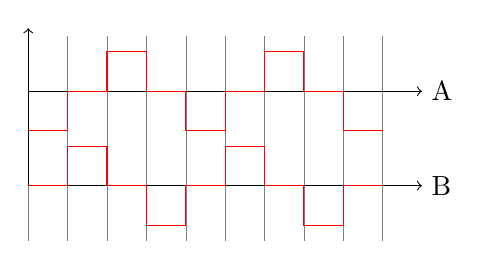
\begin{tikzpicture}
        % Hilfslinien
        \foreach \i in {0, 0.5, ..., 4.5}
        {
            \draw[ultra thin, gray] (\i, 1.9) -- (\i, -0.7);
        }
        % Achsen
    	\draw[->]	(0, 0) -- (0, 2);
    	\draw[->]	(0, 1.2) -- (5, 1.2) node[right]{A};
    	\draw[->]	(0, 0) -- (5, 0) node[right]{B};
        % Kurven
        \draw[red] 
            (0     ,0.7) --
            (0.5   ,0.7) --
            (0.5   ,1.2) --
            (1     ,1.2) --
            (1     ,1.7) --
            (1.5   ,1.7) --
            (1.5   ,1.2) --
            (2     ,1.2) --
            (2     ,0.7) --
            (2.5   ,0.7) --
            (2.5   ,1.2) --
            (3     ,1.2) --
            (3     ,1.7) --
            (3.5   ,1.7) --
            (3.5   ,1.2) --
            (4     ,1.2) --
            (4     ,0.7) --
            (4.5   ,0.7);
        \draw[red] 
            (0      ,0) --
            (0.5    ,0) --
            (0.5    ,0.5) --
            (1      ,0.5) --
            (1      ,0) --
            (1.5    ,0) --
            (1.5    ,-0.5) --
            (2      ,-0.5) --
            (2      ,0) --
            (2.5    ,0) --
            (2.5    ,0.5) --
            (3      ,0.5) --
            (3      ,0) --
            (3.5    ,0) --
            (3.5    ,-0.5) --
            (4      ,-0.5) --
            (4      ,0) --
            (4.5    ,0) ;
    	\end{tikzpicture}
    	\caption{Vollschritt}
    	\label{fig:vollschritt}
    \end{figure}
    
    \begin{figure}[H]
     	\centering
     	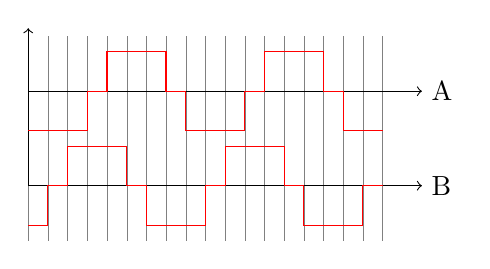
\begin{tikzpicture}
        % Hilfslinien
        \foreach \i in {0, 0.25, ..., 4.5}
        {
            \draw[ultra thin, gray] (\i, 1.9) -- (\i, -0.7);
        }
        % Achsen
    	\draw[->]	(0, 0) -- (0, 2);
    	\draw[->]	(0, 1.2) -- (5, 1.2) node[right]{A};
    	\draw[->]	(0, 0) -- (5, 0) node[right]{B};
        % Kurven
        \draw[red] 
            (0     ,0.7) --
            (0.75   ,0.7) --
            (0.75   ,1.2) --
            (1     ,1.2) --
            (1     ,1.7) --
            (1.75   ,1.7) --
            (1.75   ,1.2) --
            (2     ,1.2) --
            (2     ,0.7) --
            (2.75   ,0.7) --
            (2.75   ,1.2) --
            (3     ,1.2) --
            (3     ,1.7) --
            (3.75   ,1.7) --
            (3.75   ,1.2) --
            (4     ,1.2) --
            (4     ,0.7) --
            (4.5   ,0.7);
        \draw[red] 
            (0      ,-0.5) --
            (0.25   ,-0.5) --
            (0.25   ,0) --
            (0.5    ,0) --
            (0.5    ,0.5) --
            (1.25   ,0.5) --
            (1.25   ,0) --
            (1.5    ,0) --
            (1.5    ,-0.5) --
            (2.25   ,-0.5) --
            (2.25   ,0) --
            (2.5    ,0) --
            (2.5    ,0.5) --
            (3.25   ,0.5) --
            (3.25   ,0) --
            (3.5    ,0) --
            (3.5    ,-0.5) --
            (4.25   ,-0.5) --
            (4.25   ,0) --
            (4.5    ,0) ;
     	\end{tikzpicture}
     	\caption{Halbschritt}
     	\label{fig:halbschritt}
    \end{figure}
    \begin{figure}[H]
    	\centering
    	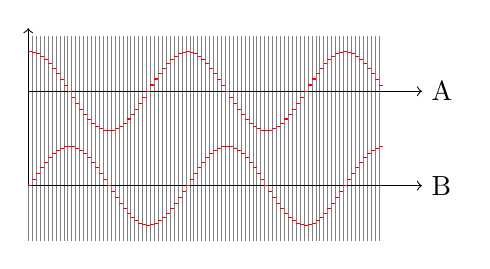
\begin{tikzpicture}
        % Hilfslinien
        \foreach \i in {0, 0.05, ..., 4.5}
        {
            \draw[ultra thin, gray] (\i, 1.9) -- (\i, -0.7);
        }
        % Achsen
    	\draw[->]	(0, 0) -- (0, 2);
    	\draw[->]	(0, 1.2) -- (5, 1.2) node[right]{A};
    	\draw[->]	(0, 0) -- (5, 0) node[right]{B};
        % Kurven
        \foreach \i in {0, 0.05, ..., 4.5}
        {
            \draw[red] (\i, {0.5*sin(180*\i)})          -- (\i+0.05, {0.5*sin(180*\i)});
            \draw[red] (\i, {0.5*sin(180*\i+(90))+1.2}) -- (\i+0.05, {0.5*sin(180*\i+(90))+1.2});
        }
    	\end{tikzpicture}
    	\caption{Mikroschritt}
    	\label{fig:mikroschritt}
    \end{figure}
    Eine Phase sind jeweils die zusammengeschalteten Statorwicklungen. Der 
    unipolare Schrittmotor besteht aus vier Phasen. Ein Elektromagnet besteht 
    aus zwei Phasen, welche gegenseitig gewickelt sind. So kann vermieden 
    werden, dass der Stromfluss durch die Wicklung gedreht werden muss. Der 
    Bipolare Schrittmotor besteht aus nur zwei Phasen. Es muss mit einer 
    Brückenschaltung die Richtung des Stromes gedreht werden. In den meisten 
    Anwendungen werden Bipolare Schrittmotoren verwendet, da ein bipolarer 
    Schrittmotor ein grössseres Drehmoment erzeugt als ein gleich grosser 
    unipolarer Schrittmotor. Die beiden Betriebsarten sind in der 
    \autoref{fig:uniVsbi} ersichtlich. 
    \begin{figure}[H]
       	\centering
       	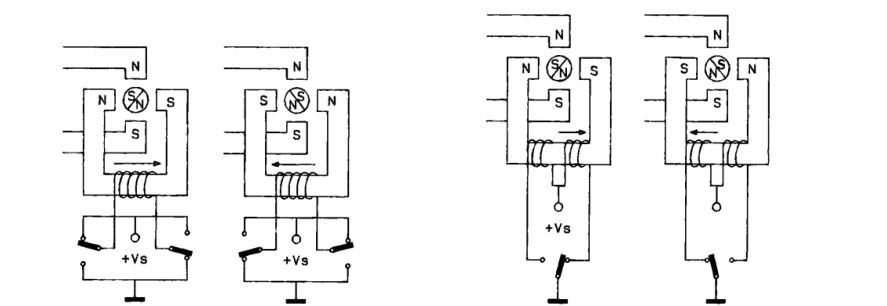
\includegraphics[width=12cm]{\EtPath/Bilder/uniVsbi.jpg}
       	\caption{bipolarer und unipolarer Betrieb}
       	\label{fig:uniVsbi}
    \end{figure}
    
       
    

	\newpage
	\ifSTANDALONE
\section{Stepper Motoransteuerung}
\fi
\ifEMBED
\subsection{Stepper Motoransteuerung}
\fi

\ifEMBED
    % Dieses Kapitel ist eine Zusammenarbeit der Gruppen \BLDCTeams. 
    \BLDCcollab
\fi
    \ifSTANDALONE
    \subsection{Grundsätzliches zur Ansteuerung}\label{subsec:Ansteuerung}
    \fi
    \ifEMBED
    \subsubsection{Grundsätzliches zur Ansteuerung}\label{subsec:Ansteuerung}
    \fi
    	Grundsätzlich besteht die Ansteuerung aus drei Teilen, wie in \autoref*{fig:ansteuerung} gezeigt. 
    	\begin{figure}[H]
    		\centering
    		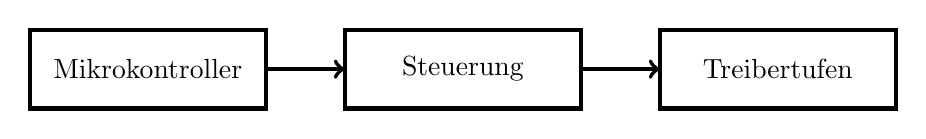
\begin{tikzpicture}
    		\draw[line width=1.5pt](0, 0) rectangle node{Mikrokontroller} (3, 1)  ;
    		\draw[line width=1.5pt, ->]	(3, 0.5) -- (4, 0.5);
    		\draw[line width=1.5pt](4, 0) rectangle node{Steuerung}(7, 1);
    		\draw[line width=1.5pt, ->]	(7, 0.5) -- (8, 0.5);
    		\draw[line width=1.5pt](8, 0) rectangle node{Treibertufen}(11, 1);
    		\end{tikzpicture}
    		\caption{Komponenten der Ansteuerung eines Schrittmotores}
    		\label{fig:ansteuerung}
    	\end{figure}
        Um die Ansteuerung zu realisieren, gibt es eine Vielzahl von integrierten Schaltkreisen. Diese unterscheiden sich wie folgt: 
        \begin{itemize}
        	\item \textbf{Interfaces:} Einzelanschlüsse, einfache Busschnittstellen oder Mikrokontrollerschnittstellen wie SPI, II2
        	\item \textbf{Steuerfunktionen:} Einzelne Schritte oder Bewegungsabläufe (Motion Control Functiona)
        	\item \textbf{Schaltungsintegration:} Steuerung und Treiberstufe als getrennte Schaltkreise, oder in einem Schaltkreis zusammengefasst. 
        \end{itemize}
        Der gewählte integrierte Schaltkreis ist der L6480 von STMicroelectronics. Dieser wird über die SPI Schnittstelle gesteuert und besitzt eine Motion Contol Engine. Die Treiberstufe wird extern realisiert. (Vgl. Kapitel \ref{sec:L6480} 
        
    \ifSTANDALONE
    \subsection{Treiberstufe}
    \fi
    \ifEMBED
    \subsubsection{Treiberstufe}
    \fi 
    	Wird ein Schrittmotor unipolar betrieben, so können die vier Wicklungen direkt mit Leistungsstufen angesteuert werden. Für den bipolaren Betrieb benötigt man für beide Wicklungen je eine H- Brücke. Die einfachste Methode ist es, den Strom nur durch den Wicklungswiderstand zu begrenzen. Der Nachteil ist, dass die Zeitkonstante durch den Wicklungswiderstand und der Induktivität bestimmt ist, und so bei höheren Schrittfrequenzen der gewünschte Strom und damit das Drehmoment nicht mehr erreicht wird. Deshalb wird ein zusätzlicher Vorwiderstand in Serie geschaltet, und so die Zeitkonstante verkleinert. Typische Verhältnisse sind vierfacher- oder fünffacher Widerstand, was eine vierfache bzw. fünffache Speisespannung voraussetzt. Diese Methode wiederum führt zu einer höheren Verlustleistung in den Widerständen. Im Ruhezustand ist es sinnvoll, den Strom soweit zu senken, dass das Haltemoment nicht unterschritten wird. Eine Spannungsumschaltung hat den weiteren Vorteil, dass so beim Anfahren eine steilere Stromkurve erreicht werden kann. (Vgl. \autoref{fig:spannungsumschaltung})
    	 \begin{figure}
    	 	\centering
    	 	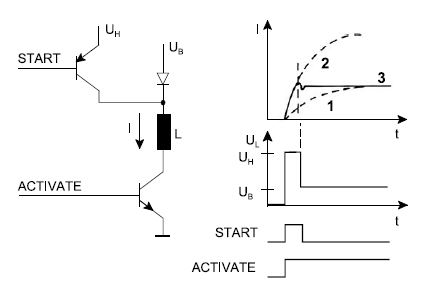
\includegraphics[width=8cm]{\EtPath/Bilder/spannungsumschaltung.JPG}
    	 	\caption{Spannungsumschaltung}
    	 	\label{fig:spannungsumschaltung}
    	 \end{figure}
    	Der Schrittmotor kann alternativ auch stromgesteuert betrieben werden. Dabei folgt der Stromverlauf dem Verlauf einer Referenzspannung (Sollwert). Der Stromverlauf wird auf den Sollwert geregelt. Die Betriebsspannung muss so nicht stabilisiert werden. \label{stromgesteuert} 
	
	
		
	\newpage
	\ifSTANDALONE
    \section{Stepper Driver L6480} \label{sec:L6480}
\fi
\ifEMBED
    \subsection{Stepper Driver L6480} \label{sec:L6480}
\fi
\ifEMBED
    % Dieses Kapitel ist eine Zusammenarbeit der Gruppen \BLDCTeams. 
    \BLDCcollab
\fi
Wie bereits im Kapitel \ref*{subsec:Ansteuerung} erwähnt, wird der L6480 von STMicroelectronics verwendet. 

\ifSTANDALONE
    \subsection{Funktionsbeschreibung}
\fi
\ifEMBED
    \subsubsection{Funktionsbeschreibung}
\fi
    Diese Schrittmotorensteuerung ist für den Betrieb von zweiphasigen (Vgl. 
    Kpaitel \ref{wirkungsweise}) Schrittmotoren mit Mikrosteps (Vgl. Kapitel 
    \ref{wirkungsweise}) geeignet. Der L6480 erreicht eine maximale Auflösung 
    von einem 1/128 Schritt. Die Steuerung generiert intern die PWM- Signale 
    für die Motorenansteuerung. Alternativ kann auch mit Vollschritten oder 
    Halbschritten gearbeitet werden. Die beiden H- Brücken werden extern mit 
    N-Kanal MOSFETs realisiert. Es können Bewegungsprofile konfiguriert 
    werden, so dass die Motoren definiert anfahren, abbremsen oder ein Punkt 
    direkt angefahren werden kann. So kann der Aufwand bei der 
    Mikrocontrollerprogrammierung verringert werden. Die Befehle werden über 
    eine SPI- Schnittstelle übertragen. Die absolute Position ist in einem 22- 
    Bit Register gespeichert. Der Bereich liegt dementsprechend zwischen 
    \(-2^{21}\) und \(2^{21}-1\). \cite{Datasheet:L6480} 

\ifSTANDALONE
    \subsection{Schnitstelle}
\fi
\ifEMBED
    \subsubsection{Schnittstelle}
\fi
Der steuernde Mikrocontroller benötigt 8 Pins für die Kommunikation mit dem 
L6480 \cite{Datasheet:L6480} : 
\begin{table}[h!]
    \begin{zebralongtable}{l l p{7cm}}
        \rowcolor{gray}\textbf{Pin} &
            \textbf{IO} &
            \textbf{Funktion} \\
        $\overline{FLAG}$ &
            Output (Open Drain) &
            Wird bei einem Fehler intern auf GND gezogen. \\
        $\overline{BUSY}$ / SYNC &
            Output (Open Drain) &
            Wird während dem Ausführen eines Befehls intern auf GND gezogen.\\
        $\overline{STBY / RESET}$ &
            Input &
            Standby- und Resetmodus, falls extern GND anliegt. \\
        STCK &
            Input &
            Im Step-Clock- Mode führt jede positive Flanke an diesem Pin zu einem 
                Schritt. \\
        \rowcolor{gray}\textbf{SPI} & & \\
        $\overline{CS}$ &
            Input &
            Chip Select: Falls extern GND anliegt, startet die Kommunikation. Um 
                die Kommunikation zu beenden, muss $\overline{CS}$ extern auf High 
                gehalten werden. \\
        CK &
            Input &
            Serial Clock: Synchronisierung der Kommunikation. \\
        SDO &
            Output &
            Slave Data Out: Daten für den Mikrocontroller. \\
        SDI &
            Input &
            Slave Data In: Befehle und Daten für den L6480. \\
    \end{zebralongtable}
    \caption{Schnittstelle des Treibers L6480}
    \label{Schnittstelle}
\end{table}
%\begin{longtable}{l l p{7cm}} \toprule
%    \textbf{Pin}    & \textbf{IO}   & \textbf{Funktion} \\
%    \midrule
%    \endhead
%    \multicolumn{3}{l}{\emph{Fortsetzung auf nächster Seite}} \\ \bottomrule \endfoot \endlastfoot          
%    \textbf{IO}\\ \addlinespace
%    %\cmidrule{1-1}
%    $\overline{FLAG}$& Output               & Wird bei einem Fehler intern auf GND gezogen. \\ \addlinespace
%    $\overline{BUSY}$ / SYNC & Output       & Wird während dem Ausführen eines Befehls intern auf GND gezogen.\\ \addlinespace
%    $\overline{STBY / RESET}$& Input        & Standby- und Resetmodus, falls extern GND anliegt. \\ \addlinespace
%    STCK            & Input         & Im Step-Clock- Mode führt jede positive Flanke an diesem Pin zu einem Schritt. \\ \addlinespace
%    %\cmidrule{1-1}
%    \textbf{SPI}\\ \addlinespace
%    %\cmidrule{1-1}
%    $\overline{CS}$ & Input         & Chip Select: Falls extern GND anliegt, startet die Kommunikation. Um die Kommunikation zu beenden, muss $\overline{CS}$ extern auf High gehalten werden. \\ \addlinespace
%    CK              & Input         & Serial Clock: Synchronisierung der Kommunikation. \\ \addlinespace
%    SDO             & Output        & Slave Data Out: Daten für den Mikrocontroller. \\ \addlinespace
%    SDI             & Input         & Slave Data In: Befehle und Daten für den L6480. \\ \addlinespace
%    \bottomrule
%    \\
%    \caption{Schnittstelle} 
%    \label{Schnittstelle}
%\end{longtable} 

\ifSTANDALONE  
    \newpage 
    \subsection{Typical Application}
\fi
\ifEMBED
    \subsubsection{Typical Application}
\fi
\begin{figure}[h]
    \centering
    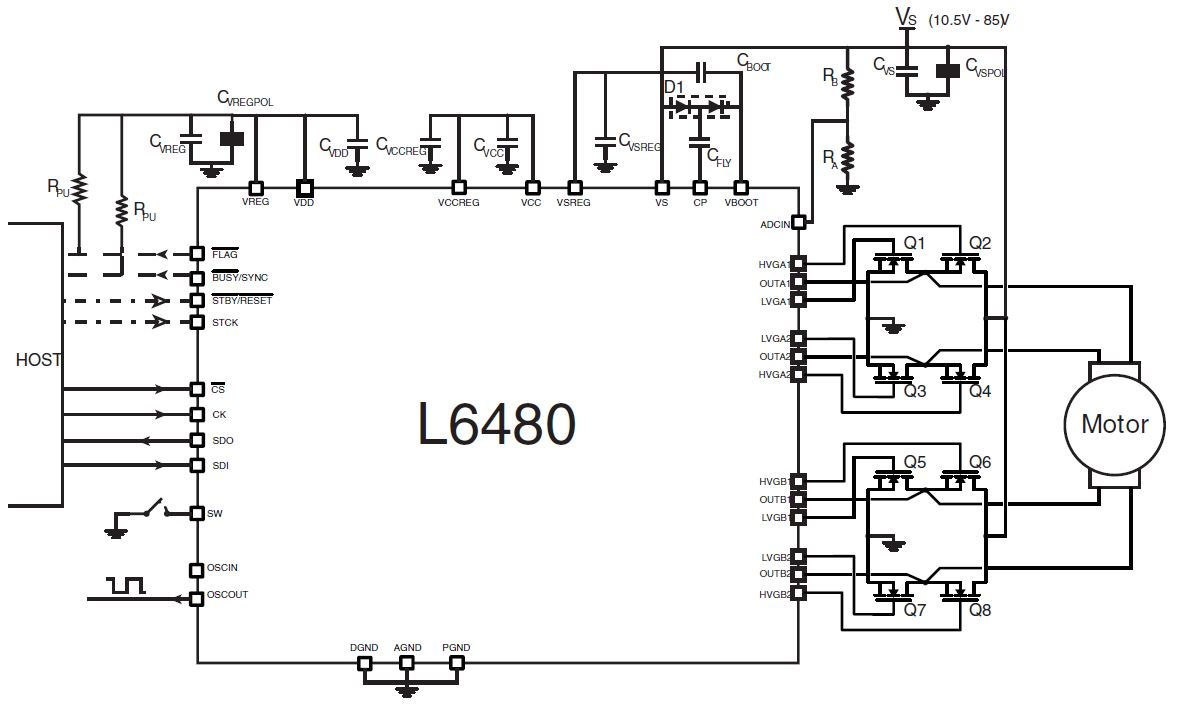
\includegraphics[width=12cm]{\EtPath/Bilder/typicalApp.jpg}
    \label{fig:typApp}
    \caption[Typical Application]{Typical Application \cite{Datasheet:L6480}}
\end{figure}

	\newpage
	\ifSTANDALONE
\section{Ausblick}
\fi
\ifEMBED
\subsection{Ausblick}
\fi
	In einem nächsten Schritt soll der L6480 bestellt werden und in einer Testschaltung getestet werden. Weiter soll ein Schema und ein Layout geplant und produziert werden, welche alle Teammitglieder in ihrem Projekt verwenden können, falls sie dies benötigen. 
	\newpage
	\setlength\bibitemsep{1.5\itemsep}
%Folgende Zeile auskommentieren, damit nur gebrauchte Literatur erscheint
\nocite{*}
\bibliography{\BIBLIOGRAPHY}
%\bibliographystyle{apacite}

	\listoffigures
	\listoftables
\end{document}
